\section{Approaches}
\label{sec:methods}

Every approach produces a full request for every pod. Settings that an approach tunes, including which of its
read-outs to report, are chosen on the validation split by mean regret; the reinforcement-learning settings are
fixed and listed with the rest in \cref{app:hyper}.

\subsection{Static requests and rules}
\textbf{Static} gives every pod the same request: a training quantile of memory need and of CPU need, and no
GPU, so every GPU task fails at start and is retried on a T4.

\textbf{Rules} are what a platform team might write by hand. If the code mentions CUDA, the task gets a GPU sized
from its largest past GPU peak times a margin. Memory is the largest past peak, converted to this pod's units and
multiplied by a margin, or the static request if there is no history. CPU is the largest past peak in cores times
a margin; on a first run it falls back to the largest pool size the code declares (\code{max\_workers=},
\code{n\_jobs=} and so on), or one core.

\textbf{Rules-sized} also reads input sizes and the pod spec. With history, it takes the earlier run closest in
input size and scales its peak by the ratio of input sizes. On a first run it estimates the workload's peak as
$a + k\cdot\text{input MiB}$, with $a$ and $k$ tuned on validation first runs, and adds the staging's cost as read
from the pod spec: 48\,MiB if \code{job.py} imports boto3, and the staged bytes if the manifest says
\code{medium: Memory}. It then converts that peak into the pod's need with the accounting of
\cref{sec:accounting}. Rules-sized therefore uses the benchmark's own accounting constants (the runtime, the
boto3 footprint, the headroom), which a learned model has to infer from data.

\subsection{Gradient-boosted quantile trees}
The trees use 209 features a scheduler can compute. Twenty-seven describe the inputs and history: total bytes,
bytes by format, visible rows, column counts, array shapes, the number of earlier runs, their peaks, and the size
ratio to the closest earlier run. Another 173 mark API tokens in the code, such as \code{groupby},
\code{TfidfVectorizer} or \code{ProcessPoolExecutor}, and numeric literals such as pool sizes, layer widths and
batch sizes. Four flag CUDA use, and five flag details of a Job's pod spec (\code{kind: Job},
\code{initContainers}, \code{medium: Memory}, \code{import boto3} and \code{download\_file}).

For each axis we fit 19 quantile regressors~\citep{koenker1978quantile} with scikit-learn's
\code{HistGradientBoostingRegressor} (quantiles 0.05 to 0.95, 300 rounds, learning rate 0.06, 31 leaves) on the
base-2 log of the need, plus a classifier that predicts whether the task needs a GPU. The predicted quantiles
define a piecewise-linear CDF, and each cell's probability is the CDF mass between its edges. The fit is
deterministic. Two ablations train on Job pods only or on Flyte pods only.

\subsection{Zero-shot 27B}
A 27B-parameter Qwen instruction model, served with vLLM~\citep{kwon2023vllm}, reads the prompt shown in
\cref{app:prompt} and answers in JSON at temperature zero. We read units as Kubernetes would (so \code{2 GiB},
\code{2GB} and \code{500m} all parse) and round each value up onto the grid; an answer we cannot parse falls back
to 4\,Gi, one core and no GPU. The model writes plain-text reasoning before its answer even with thinking turned
off, so we give it up to 8,192 tokens, and we also score a variant whose decoding is constrained to the answer's
JSON schema with 256 tokens. Both are scored on a family-stratified sample of 150 runs per split, each run's Job
and Flyte pods, which leaves 130 test and 150 unseen Job pods. \Cref{sec:res-zs} compares every approach on that
same sample.

\subsection{Decision model: three pointer heads on one forward pass}
The decision model reads the prompt and scores every option on every axis in one forward pass
(\cref{fig:pointer}). The options are written out at the end of the prompt. For each axis, a small head compares
the hidden state at the prompt's last token with the hidden state at each option's last token:
\begin{equation}
s_{\text{axis}}(j) = \frac{\langle W_{q,\text{axis}}\,\mathrm{LN}(a),\ W_{k,\text{axis}}\,\mathrm{LN}(k_j)\rangle}{\sqrt{256}},\qquad
P(\text{axis}=j) = \mathrm{softmax}_j\!\big(s_{\text{axis}}(j)/T_{\text{axis}}\big).
\end{equation}
Here $a$ is the last prompt token's hidden state, $k_j$ is option $j$'s, each axis has its own affine maps
$W_q, W_k$ from 2,048 to 256 dimensions, $\mathrm{LN}$ is one shared LayerNorm, and the temperature
$T_{\text{axis}}$ minimizes validation negative log-likelihood. This is a pointer
mechanism~\citep{vinyals2015pointer} over option tokens: the model reads the candidates in its context, so the
same heads work for any option list written in the same format.

\begin{figure}[tbp]
\centering
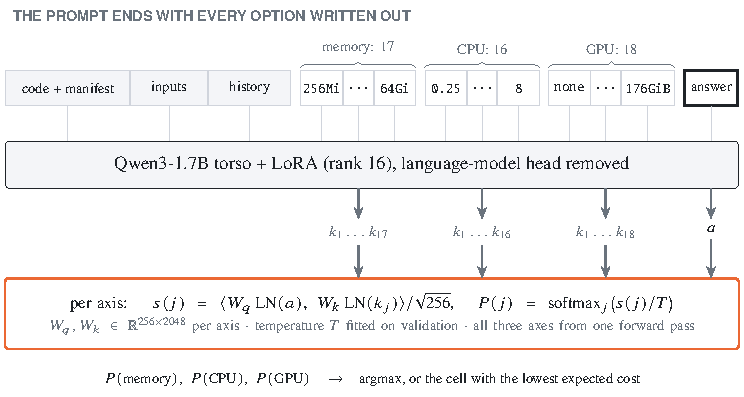
\includegraphics[width=\linewidth]{figures/diagrams/pointer.pdf}
\caption{The pointer decision model. Every prompt ends with the same options block and answer instruction, so
each option's last token sits at a fixed offset from the end, and one forward pass gives a distribution on all
three axes.}
\label{fig:pointer}
\end{figure}

The torso is Qwen3-1.7B~\citep{qwen3} without its language-model head, adapted with LoRA~\citep{hu2022lora}
(rank 16, $\alpha$ 32) on every projection of every layer. Prompts are cut from the left at 3,072 tokens, a length
no evaluated prompt reaches. The loss is the sum of the three axes' cross-entropies, leaving out memory and CPU for
GPU tasks. Training uses at most 5,000 rows per corpus and pod type, 27,936 rows in all, for one epoch with
micro-batches of 8, two accumulation steps, and AdamW at $2\times10^{-4}$ for the adapters and $10^{-3}$ for the
heads, on one NVIDIA L4. Two ablations train on one pod type only, on half the rows for two epochs, so that all
three variants take the same number of steps; each is calibrated on its own pod type's validation rows. The two
pod types are drawn independently, so the model trained on both sees about 40\% more distinct workloads than
either ablation.

\subsection{Turning a distribution into a request}
The trees, the decision models and the pools all give a distribution on each axis, and we read each one out in
two ways. The \emph{argmax} read-out takes the most likely cell on each axis. The \emph{decoded} read-out first
decides whether to give a GPU, choosing none when $P(\text{none})$ is at least a threshold $\theta$ tuned on
validation, and otherwise the most likely GPU cell. For memory it picks the cell with the lowest expected cost,
$\arg\min_m \sum_j C[m,j]\,P(j)$, where $C[m,j]$ is RightSizeMem's memory cost of requesting cell $m$ for a run
that needs cell $j$, retries included (a fixed matrix, not the per-run simulator). For CPU it picks the cell most
likely to fall within 25\% of the busiest window. An OOM costs a retry, so decoding leans toward asking for more
memory. For each model, validation decides which read-out the leaderboard reports (\cref{tab:readouts}).

\subsection{Reinforcement learning against the cost model}
Matching the label misses two things the cost model cares about. The axes interact: memory and CPU are free on
a GPU node, while a GPU is the most expensive mistake on a CPU node. And asking for too little costs more than
asking for too much. The RL approach starts from the decision model and maximizes the cost model's reward
(\cref{alg:grpo}). Because the policy is three categorical distributions, a group of 16 joint requests comes from
one forward pass and no text is generated. Advantages are normalized within each group as in
GRPO~\citep{shao2024deepseekmath}, and each batch takes one on-policy step, so the update is REINFORCE with a
group baseline and an exact KL penalty to the supervised model; there is no clipped ratio. It trains on 6,000
training prompts, about half of them unseen by the supervised model, for one epoch with a KL coefficient of 0.05
and the reward capped at 20.

The fitted temperatures of every RL model sit at or near the top of the search range (5.0), so its decoded
read-out is set by that bound. The RL policy moves probability away from the label cell on purpose, so
calibrating it against the label is the wrong target, and validation prefers its argmax read-out.

\begin{figure}[tbp]
\begin{lstlisting}
pi_ref = the supervised model's distributions, computed once before any update
for each batch of 8 prompts:
    one forward pass -> pi(.|x) on each axis
    sample K = 16 joint requests a^k = (m, c, g) from the three heads        # no text is generated
    r^k = - min( cost(x, a^k) / label_cost(x), 20 )                            # the benchmark's simulator
    A^k = (r^k - mean_k r) / (std_k r + 1e-3)                                  # group-normalized
    L   = - mean_k[ A^k * sum_{axis in S(x)} log pi(a^k_axis | x) ] + 0.05 * sum_{axis in S(x)} KL(pi || pi_ref)
    S(x) = {gpu} for a GPU task, else all three axes
\end{lstlisting}
\caption{RL without generation. The reward divides by a fixed cost per run, so the best request for each run is
the cheapest one whichever denominator is used. The KL term is exact over the categorical distributions.}
\label{alg:grpo}
\end{figure}

\subsection{Opinion pools}
The trees and the language models make different mistakes. The trees read numbers exactly and have nothing to go
on for code they have never seen; the language models read code well and treat numbers as tokens. A logarithmic
opinion pool~\citep{genest1986pools} combines their calibrated distributions on each axis:
\begin{equation}
p_{\text{pool}}(j) \propto p_{\text{trees}}(j)^{w}\,p_{\text{LM}}(j)^{1-w}.
\end{equation}
One weight $w$ is shared across the three axes and tuned on validation together with $\theta$, for the decoded
read-out; nothing is retrained. A model trained on one pod type is pooled with trees trained on the same pod type.

\subsection{A novelty gate}
In our first release, the pooled RL model read by argmax was the best approach on familiar code and one of the
worst on new code, while the RL model read out by decoding was the reverse. The gate sends each pod to one or the
other by its distance from the training data:
\begin{equation}
s(x) = \tfrac{1}{10}\textstyle\sum_{i=1}^{10}\lVert z(x) - z(x_{(i)})\rVert_2,\qquad
\text{request} = \begin{cases}\text{pool}\times\text{RL, argmax} & \text{if } s(x)\le\tau,\\ \text{RL, decoded} & \text{otherwise.}\end{cases}
\end{equation}
Here $z$ standardizes the trees' 209 features by their training mean and standard deviation, $x_{(i)}$ are the ten
nearest training pods, and $\tau$ is the 95th percentile of $s$ on validation. Validation has familiar families
only, so it cannot tune the gate: the threshold sends 5\% of familiar pods to the RL model by construction, and
validation regret falls steadily as fewer pods are routed. We chose the members, the signal and the threshold after
seeing the first release's unseen results, and fixed them before training k8s-2 at new seeds. k8s-2 has the same
seven held-out families, so it tests whether the choice holds up after relabelling and retraining, not whether it
generalizes to new families.

Our first release divided a feature that never varied in training by $10^{-9}$, so any pod with an unseen import
landed effectively infinitely far away. Such features now keep their raw units; the old scaling remains as a
comparison. We also compare two other signals: kNN on the 27 numeric features alone, and the Jensen--Shannon
divergence between the trees' and the RL model's predictions.

\subsection{A Flyte-to-Job adapter}
A team whose history is all Flyte tasks has no Job pods to train on. The adapter shifts a Flyte-trained model's
memory distribution with the accounting of \cref{sec:accounting}: each cell's representative need $n_j$ (its
geometric middle) becomes $(n_j/1.05 - R + 48[\text{boto3}] + B[\text{tmpfs}])\times1.05$, using the manifest's
volume medium, whether \code{job.py} imports boto3, and the input sizes. CPU and GPU come from the model's own
reading of the Job's prompt. Its memory distribution can come from the model's reading of the Job's prompt (the
variant a scheduler can deploy) or of the same run's Flyte task, which a scheduler holding only a raw Job does not
have. We report both.
